\documentclass[tikz,border=2pt]{standalone}
\usepackage{amsmath}
\usetikzlibrary{arrows.meta}
\begin{document}
% Six workers (Gender, Dept), one with a missing department, counted into a 2 x 3 table:
% Female: Engineering 1, Management 0, Sales 2; Male: 1, 1, 0. The NA row is not counted (total 5).
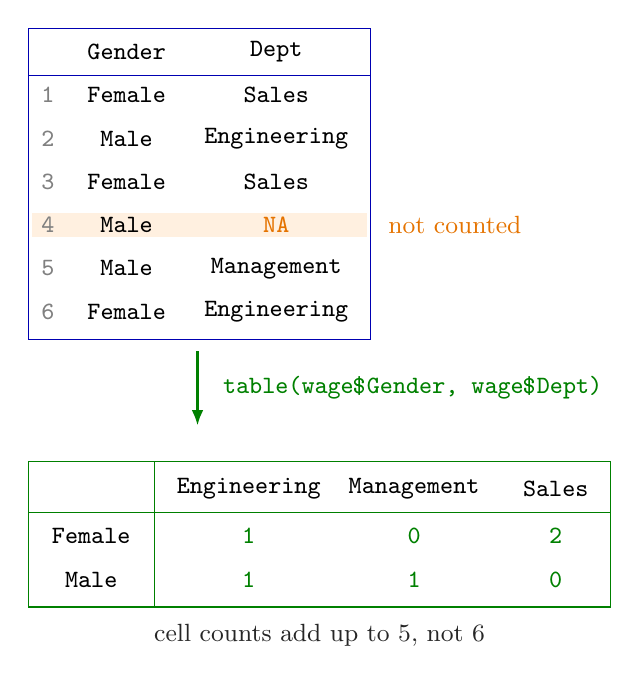
\begin{tikzpicture}[font=\small, >={Latex[length=2mm]},
  t/.style={font=\small\ttfamily},
  hd/.style={font=\small\ttfamily\bfseries}]
  % data frame
  \fill[orange!12] (-0.2,-2.05) rectangle (4.05,-2.35);
  \node[hd] at (1.0,0) {Gender}; \node[hd] at (2.9,0) {Dept};
  \draw[blue!70!black] (-0.25,0.3) rectangle (4.1,-3.65);
  \draw[blue!70!black] (-0.25,-0.3) -- (4.1,-0.3);
  \foreach \g/\d [count=\i] in {Female/Sales, Male/Engineering, Female/Sales, Male/NA, Male/Management, Female/Engineering} {
    \node[t, gray] at (0.0,-0.55*\i) {\i};
    \node[t] at (1.0,-0.55*\i) {\g};
  }
  \foreach \d [count=\i] in {Sales, Engineering, Sales, NA, Management, Engineering} {
    \ifnum\i=4
      \node[t, orange!90!black] at (2.9,-0.55*\i) {NA};
    \else
      \node[t] at (2.9,-0.55*\i) {\d};
    \fi
  }
  \node[orange!90!black, anchor=west] at (4.2,-2.2) {not counted};
  % arrow
  \draw[->, very thick, green!50!black] (1.9,-3.8) -- (1.9,-4.75);
  \node[t, green!50!black, anchor=west] at (2.1,-4.27) {table(wage\$Gender, wage\$Dept)};
  % two-way table
  \begin{scope}[yshift=-5.2cm]
    \node[hd] at (2.55,-0.35) {Engineering}; \node[hd] at (4.65,-0.35) {Management}; \node[hd] at (6.45,-0.35) {Sales};
    \draw[green!50!black] (-0.25,0) rectangle (7.15,-1.85);
    \draw[green!50!black] (-0.25,-0.65) -- (7.15,-0.65);
    \draw[green!50!black] (1.35,0) -- (1.35,-1.85);
    \node[hd] at (0.55,-0.95) {Female}; \node[hd] at (0.55,-1.5) {Male};
    \foreach \v/\x in {1/2.55, 0/4.65, 2/6.45} { \node[t, green!50!black] at (\x,-0.95) {\v}; }
    \foreach \v/\x in {1/2.55, 1/4.65, 0/6.45} { \node[t, green!50!black] at (\x,-1.5) {\v}; }
    \node[gray!30!black, anchor=north] at (3.45,-1.95) {cell counts add up to 5, not 6};
  \end{scope}
\end{tikzpicture}
\end{document}
